\begin{figure}[!htb]
    % \centering
    \Subfigure[0.49]{\includegraphics[width=1\textwidth]{figures/simulations/coll_rad/CD+_He_f-time__transition_0-1_0.001s_population_ratio.pdf}}{}{\label{fig:ROSAA-sim-coll-rad-population}}
    \hfill
    \Subfigure[0.49]{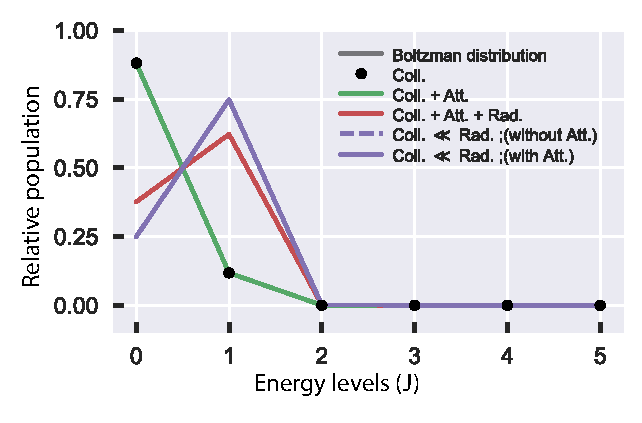
\includegraphics[width=1\textwidth]{figures/simulations/coll_rad/CD+_He_f-time__transition_0-1_0.001s_boltzman_comparision.pdf}}{}{\label{fig:ROSAA-sim-coll-rad-boltzmann}}
    
    \caption{(a) Simulated relative rotational level populations for \CD as labelled in parenthesis. The population evolves from $t=0$ (T$_{coll}=300$ K) to reach equilibrium at $t<0.5$ ms. The solid and dashed lineshapes correspond with (ON) and without (OFF) the presence of radiation for \CD \CDline transition. The radiation power is $35\ \mu$ W. (b) Compares the Boltzmann distribution at 7 K with the relative population involving only collisional process (Coll.) and, collision and radiative process (Coll. + Rad.) at $t=1$ ms.}
    \label{fig:ROSAA-sim-coll-rad-population-boltzmann}
\end{figure}
